\section{Results}
\subsection{Empirical evidence of temporal clustering}
Figure~\ref{fig:ecdf-dt-poisson} compares the empirical CDF of the
inter-event times $\Delta t_i = t_i - t_{i-1}$ with the
$\mathrm{Exp}(\hat\lambda)$ CDF, where $\hat\lambda = N/(T-t_0)$.
The empirical curve lies above the Poisson benchmark near the origin
and below it for intermediate gaps, indicating an excess of very short
inter-event times and a deficit of medium gaps. This pattern is
characteristic of aftershock clustering and already suggests that a
homogeneous Poisson process is inadequate.

\begin{figure}[t]
  \centering
  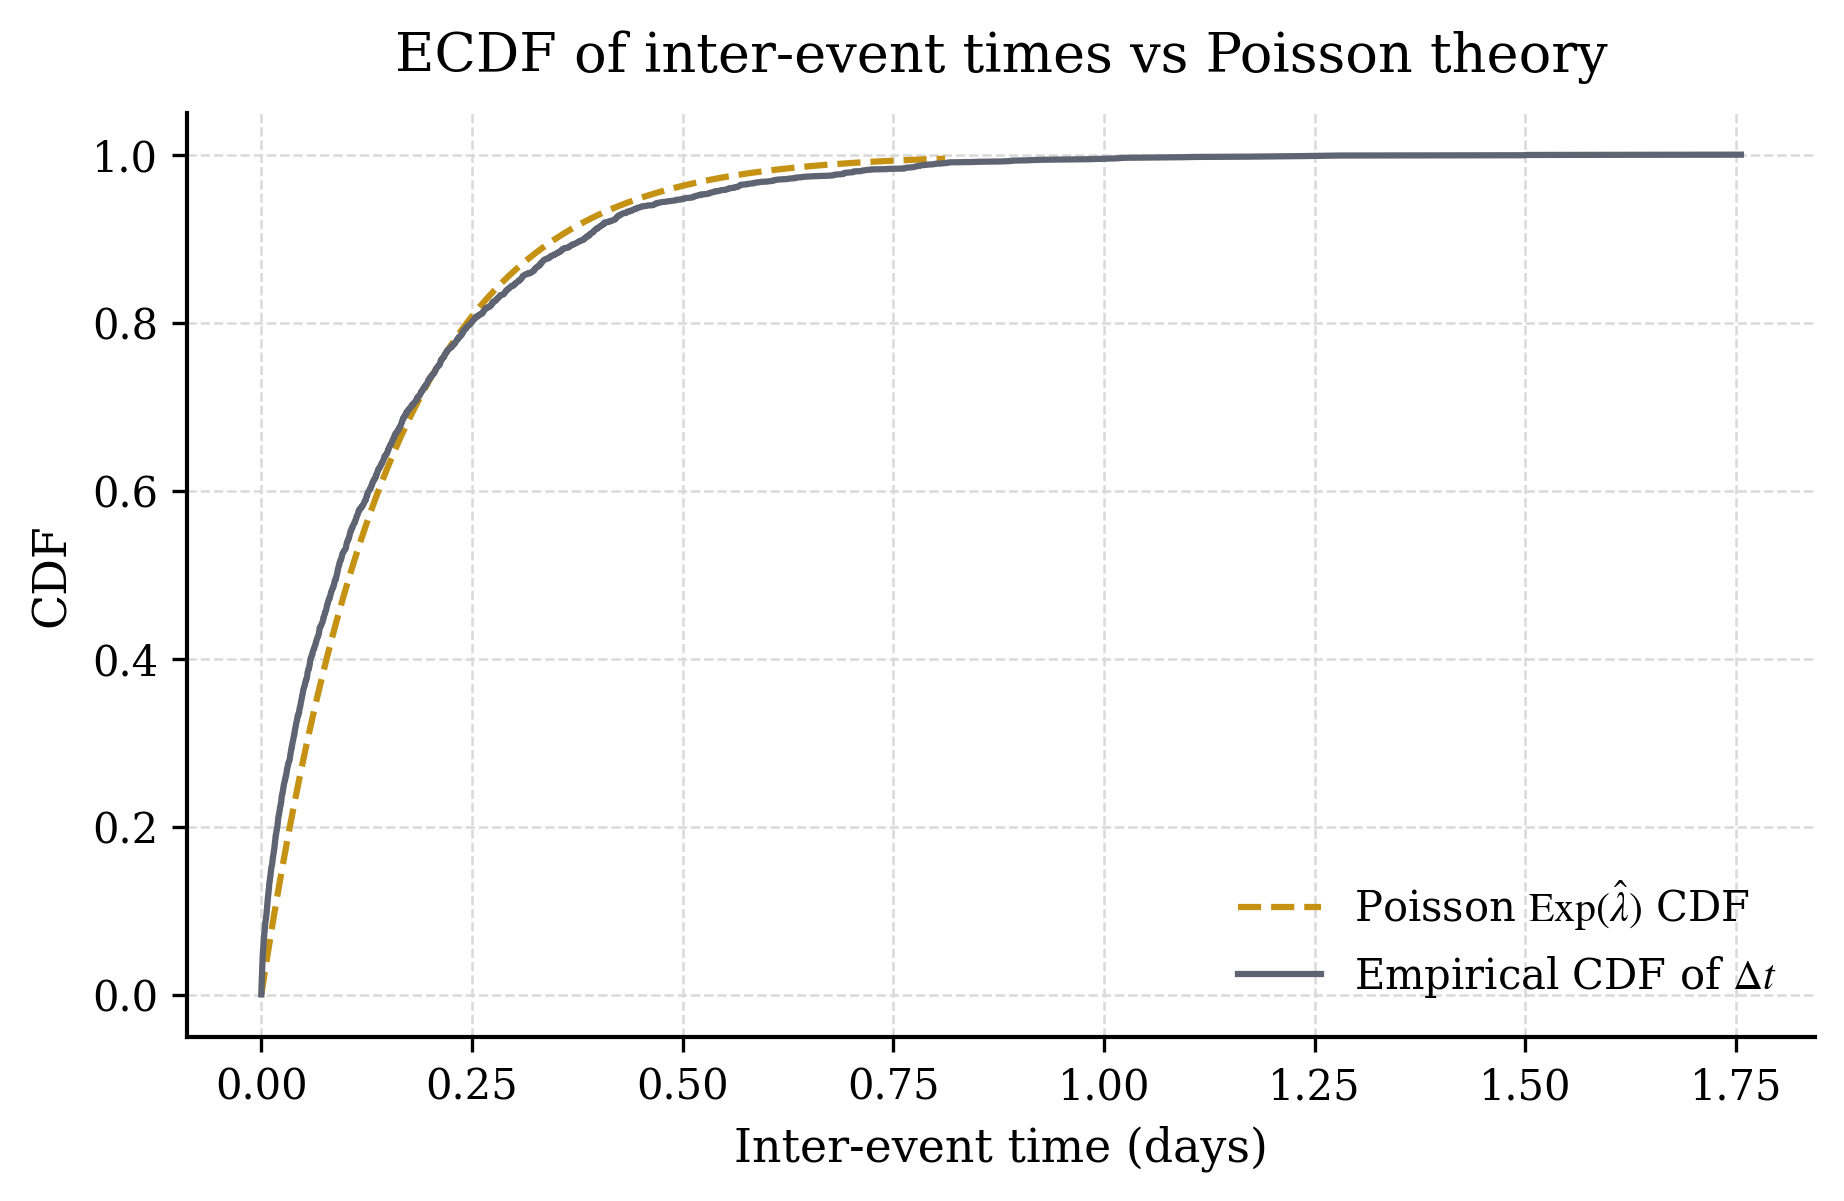
\includegraphics[width=0.8\textwidth]{plots/ecdf_dt_vs_poisson.png}
  \caption{Empirical CDF of $\Delta t_i$ (solid) against the
  $\mathrm{Exp}(\hat\lambda)$ CDF (dashed).}
  \label{fig:ecdf-dt-poisson}
\end{figure}

\subsection{Fitted models}
Table~\ref{tab:params} reports the MLE parameter estimates for all
five models. The Hawkes fits indicate substantial self-excitation, and
the marked models yield $\hat\gamma > 0$, confirming a positive
dependence of triggering strength on magnitude.
Figure~\ref{fig:intensity-full} shows the fitted conditional intensities
for the three main models: the Poisson intensity is constant, whereas
both Hawkes intensities are spiky, with the marked variant producing
sharper peaks after large earthquakes.

\begin{table}[t]
  \centering
  \caption{MLE parameter estimates.}
  \label{tab:params}
  \begin{tabular}{lc}
    \toprule
    Model & Estimates \\
    \midrule
    Poisson &
      $\hat\lambda = 6.59$ \\
    Exponential Hawkes &
      $(\hat\mu,\hat\alpha,\hat\beta) = (5.47, 9.16, 53.98)$ \\
    Power-law Hawkes &
      $(\hat\mu,\hat K,\hat c,\hat p) = (3.30, 0.05, 0.10, 1.50)$ \\
    Marked exp.\ Hawkes &
      $(\hat\mu,\hat\alpha,\hat\beta,\hat\gamma) = (5.52, 5.02, 55.85, 1.12)$ \\
    Marked power-law Hawkes &
      $(\hat\mu,\hat K,\hat c,\hat p,\hat\gamma) = (4.38, 0.067, 0.55, 5.00, 1.09)$ \\
    \bottomrule
  \end{tabular}
\end{table}

\begin{figure}[t]
  \centering
  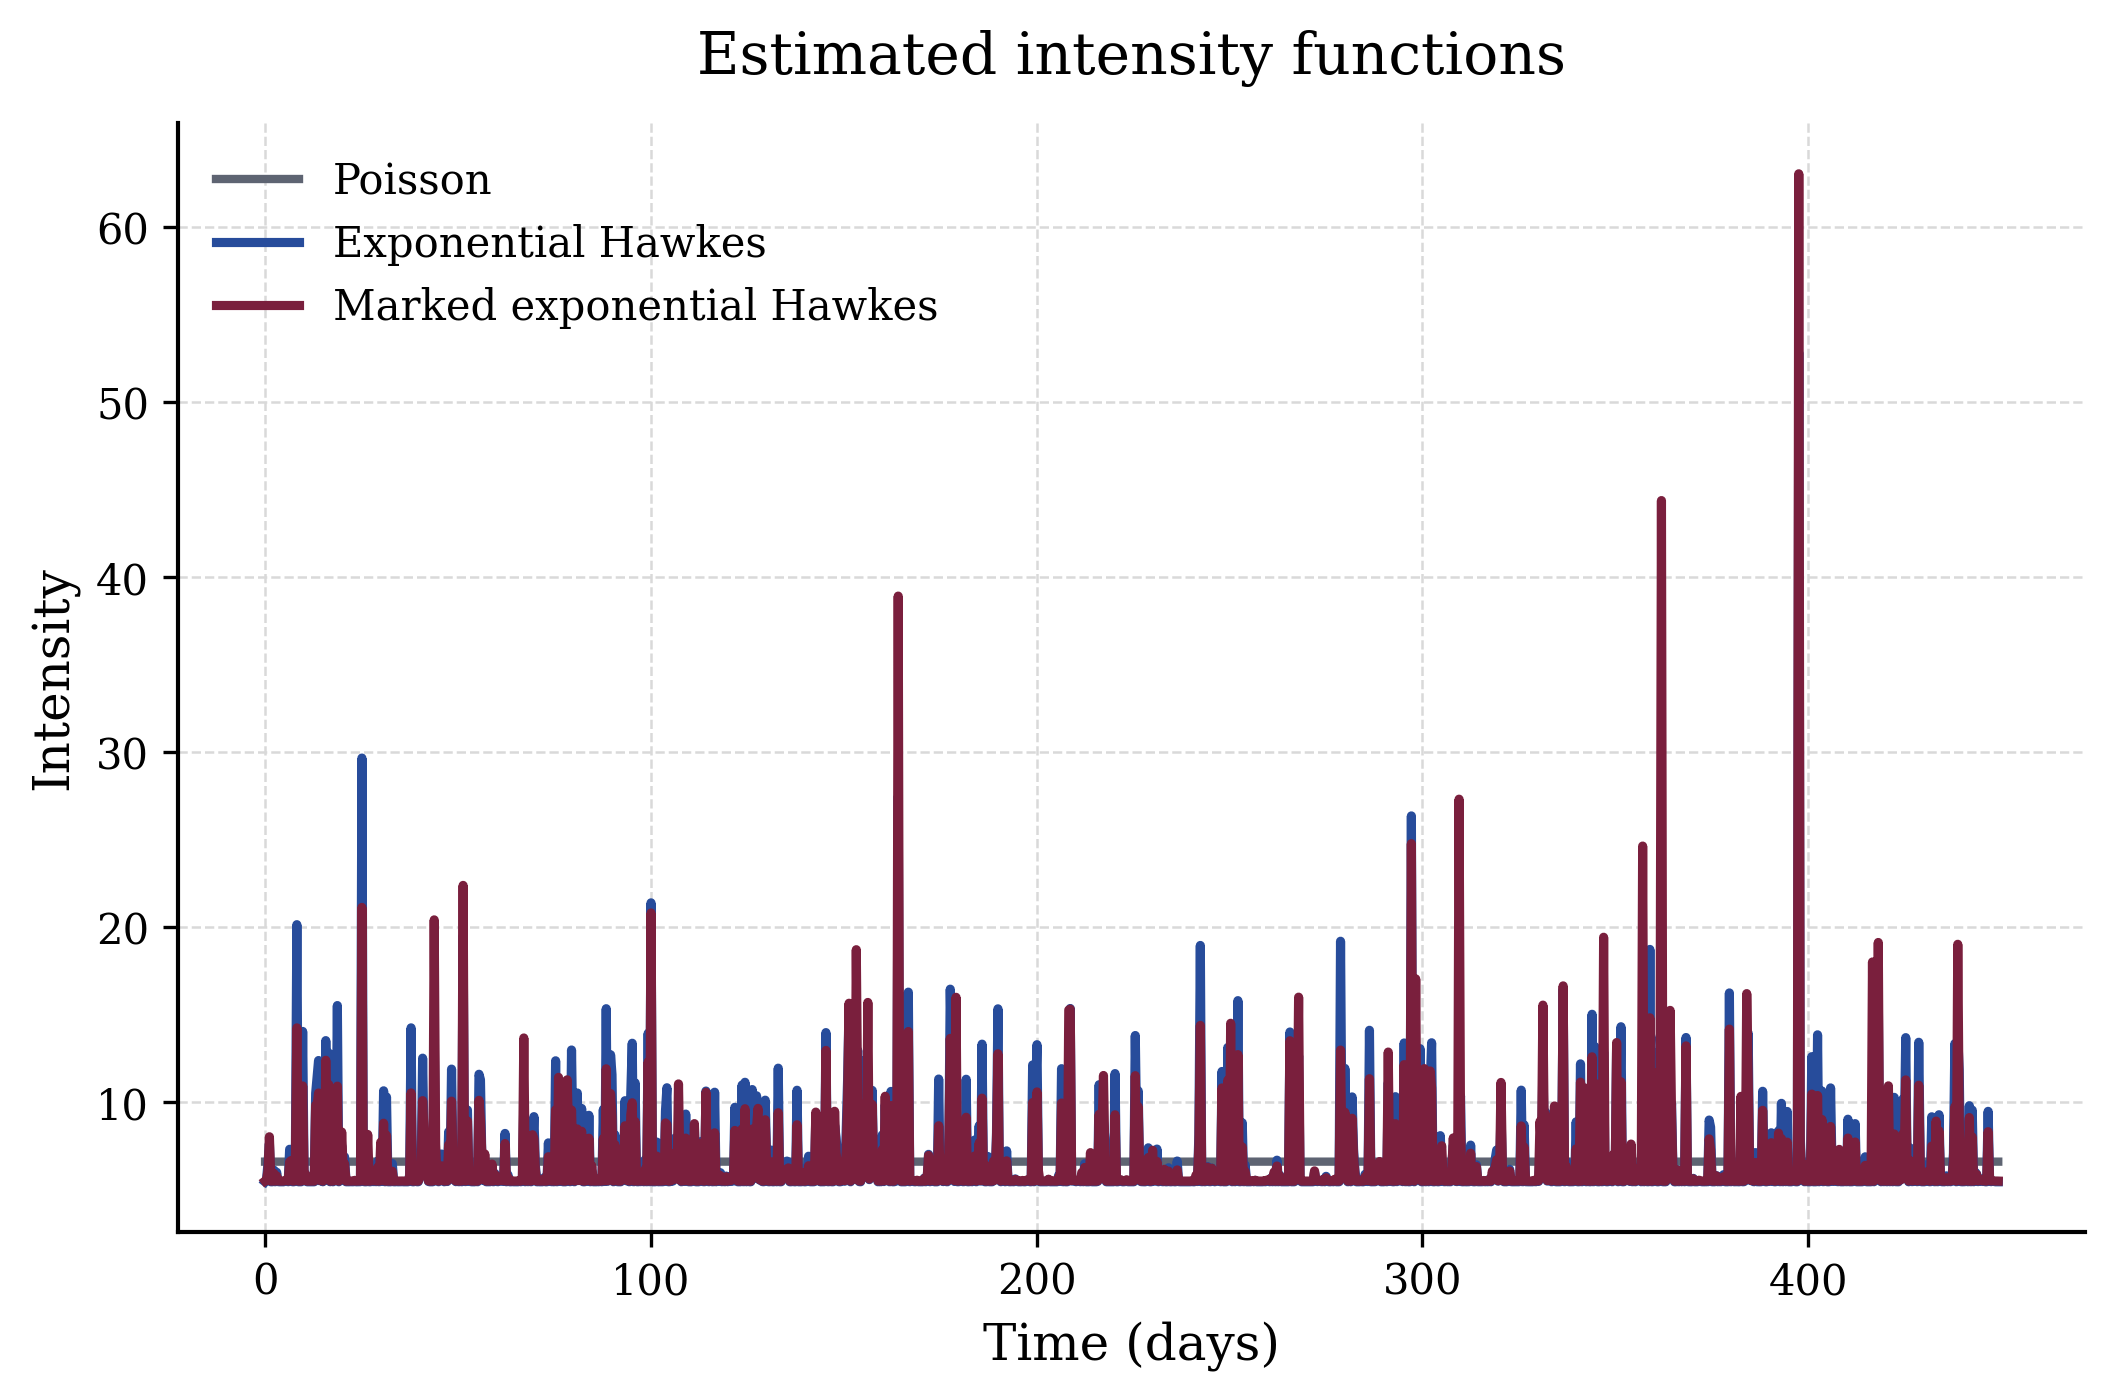
\includegraphics[width=0.8\textwidth]{plots/intensity_curves.png}
  \caption{Estimated conditional intensity functions for the Poisson,
  exponential Hawkes and marked exponential Hawkes models.}
  \label{fig:intensity-full}
\end{figure}

\subsection{Residual diagnostics}
We apply Ogata's time-rescaling theorem: under correct specification,
the rescaled gaps $\Delta\tau_i = \Lambda_{\hat\theta}(t_i) -
\Lambda_{\hat\theta}(t_{i-1})$ should be i.i.d.\ $\mathrm{Exp}(1)$.
The Poisson and power-law Hawkes models are both strongly rejected by
KS and chi-squared tests ($p < 10^{-19}$). The exponential Hawkes model
performs substantially better (KS statistic $0.022$, $p \approx 0.12$),
and the marked exponential Hawkes model provides the best agreement
(KS statistic $0.017$, $p \approx 0.39$; chi-squared $p \approx 0.07$).
Figures~\ref{fig:ks-three} and~\ref{fig:density-three} confirm this
visually: the marked exponential Hawkes residuals are nearly
indistinguishable from the $\mathrm{Exp}(1)$ benchmark, while all
other models show clear discrepancies.

\begin{figure}[t]
  \centering
  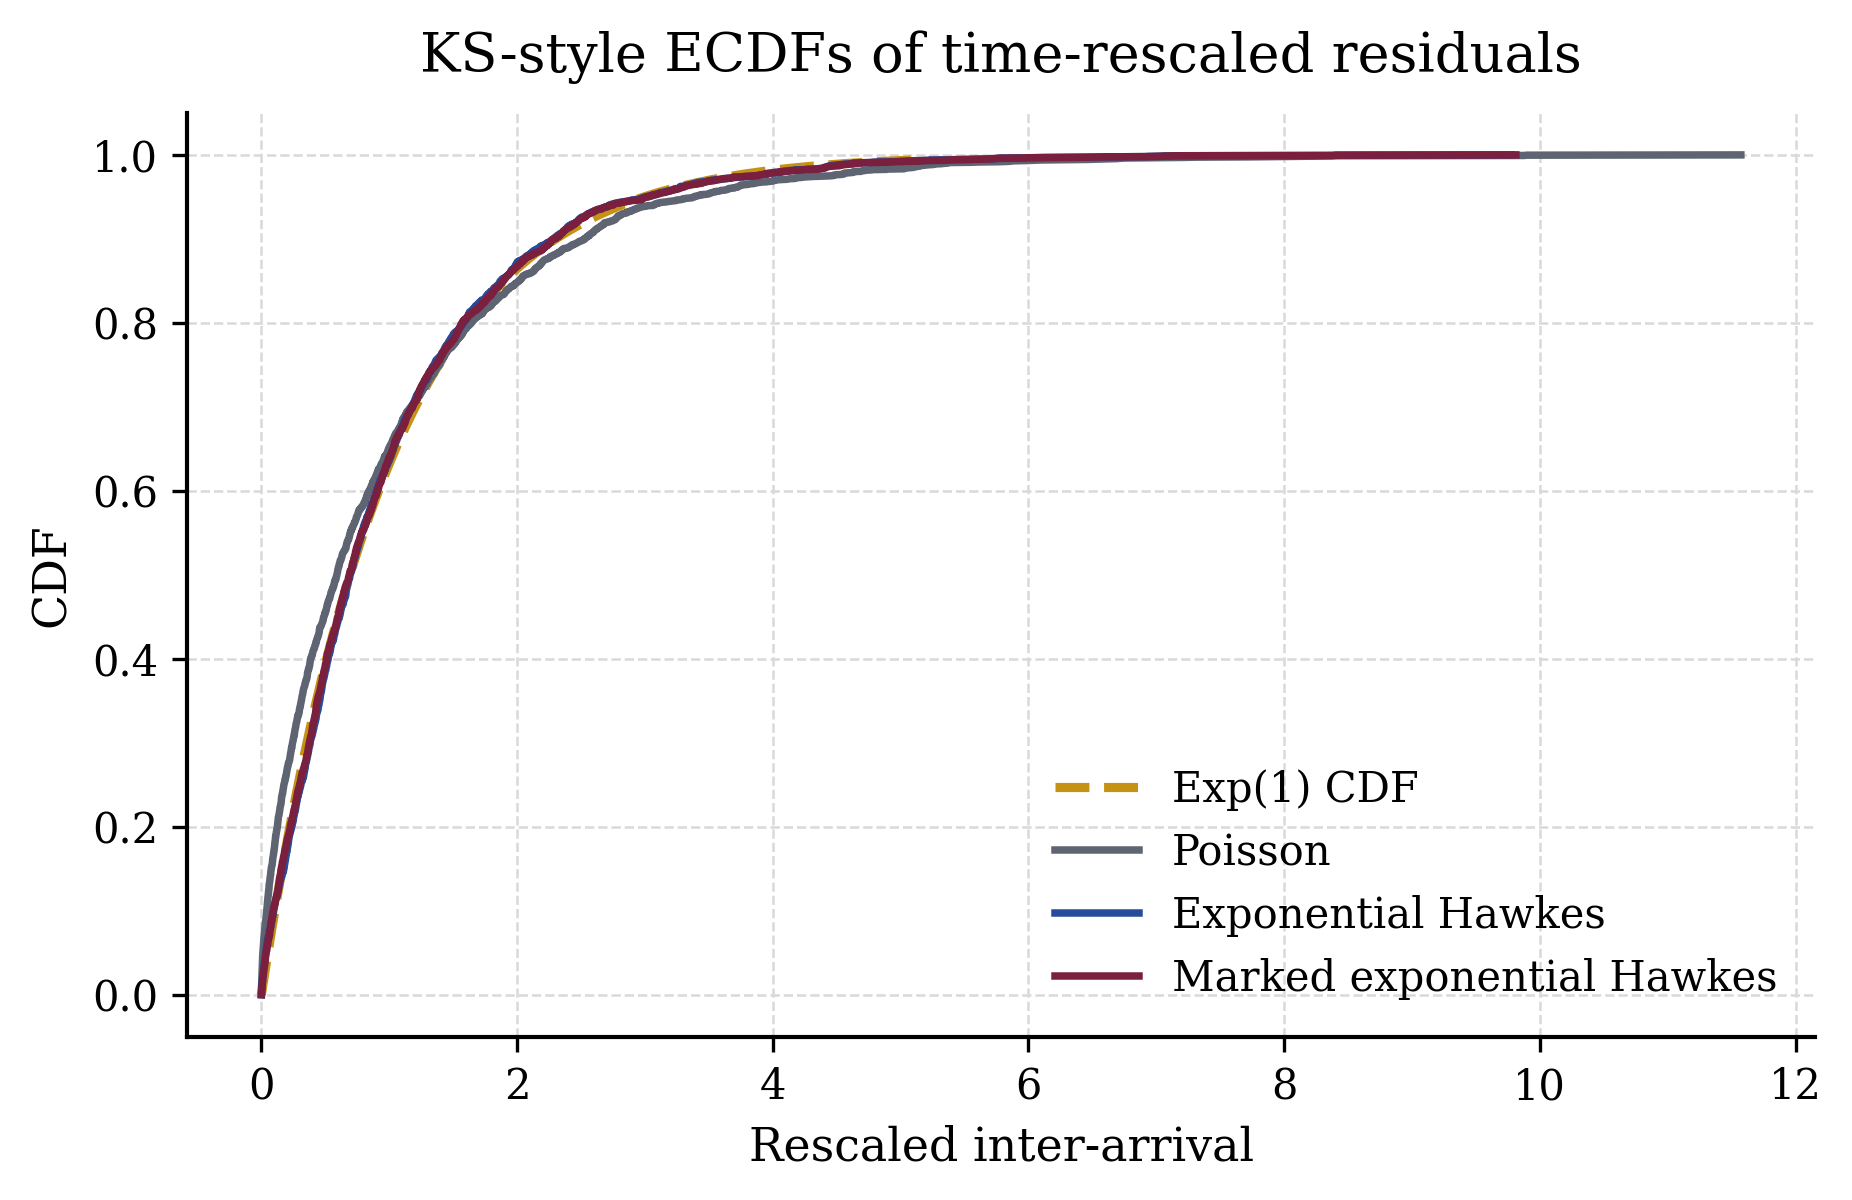
\includegraphics[width=0.8\textwidth]{plots/ks_ecdf_residuals.png}
  \caption{Empirical CDFs of the rescaled inter-arrival times against
  the $\mathrm{Exp}(1)$ CDF (dashed).}
  \label{fig:ks-three}
\end{figure}

\begin{figure}[t]
  \centering
  
\includegraphics[width=0.8\textwidth]{plots/density_residuals.png}
  \caption{Residual densities against the $\mathrm{Exp}(1)$ density
  (dashed).}
  \label{fig:density-three}
\end{figure}
